\section{Introduction}

While studying binary reduction algorithms, we tested some cases by hand. However, even small polynomials can require dozens of bit operations, so the number and size of our manual tests was severely limited, but still yielded interesting results. \\

In our tests we often spotted interesting behaviors. Some bits would cancel themselves in ways that suggested a pattern, or a change in one of the variables would lead to non-obvious changes in the number of operations. On the one hand, we knew many of those behaviors were coincidences, so attempts at extracting mathematical proofs for each of them would lead to many dead ends and wasted time. On the other hand, patterns like these were the base of many optimizations. \\

Therefore we needed a way to quickly test different parameters, and have the results be visually intuitive, in order to discern behaviors that were more likely to be useful. This chapter explains the initial process and the final tool developed. In Section~\ref{section:visual:manual} we explain how the manual tests were organized. Section~\ref{section:visual:alt} we show how the manual tests were reworked to create more visually intuitive results. Finally, Section~\ref{section:visual:final} contains some of the optimizations made for faster feedback, along with a few of the patterns observed. Section~\ref{section:visual:conclusion} concludes with some remarks. \\

\section{Manual reduction algorithm} \label{section:visual:manual}

The reduction process for polynomials in $GF(2^m)$ depends on two values: the irreducible polynomial $f(x) = x^m + x^a + \cdots + 1$, and the value to be reduced, $C(x) = \sum_{i=0}^{d} c_i x^i$, $d \geq m$. Here we focus on the case $d=2m-2$. This is a common situation that arises when $C$ is the product of two polynomials of degree less than $m$, or the square of a single polynomial of this size. \\

For example, take the irreducible trinomial $f(x) = x^7 + x^3 + 1$, and $C(x) = x^{12} + x^{10} + x^9 + x^7 + x^6 + x^3 + x^2 + 1$. We can look at $f$ and $C$ as arrays of bits (see Figure~\ref{fig:visual:table_simplest}). \\

\begin{figure}
  \centering
\begin{TAB}(e){|c|c|c|c|c|c|c|c|c|c|c|c|c|}{|c|c|c|}
\emph{$x^{12}$} & \emph{$x^{11}$} & \emph{$x^{10}$} & \emph{$x^9$} & \emph{$x^8$} & \emph{$x^7$} & \emph{$x^6$} & \emph{$x^5$} & \emph{$x^4$} & \emph{$x^3$} & \emph{$x^2$} & \emph{$x^1$} & \emph{$x^0$} \\
  &   &   &   &   & 1 & 0 & 0 & 0 & 1 & 0 & 0 & 1 \\
1 & 0 & 1 & 1 & 0 & 1 & 1 & 0 & 0 & 1 & 1 & 0 & 1
\end{TAB}
\caption{The polynomials $x^7 + x^3 + 1$, and $x^{12} + x^{10} + x^9 + x^7 + x^6 + x^3 + x^2 + 1$ seen as arrays of bits.}
\label{fig:visual:table_simplest}
\end{figure}

At this point in the research, the algorithm we were using for polynomial reduction was slightly different from the one previously shown. First, notice that $0 \equiv f \pmod f$, so we can add $f$ or any multiple to an expression maintaining the same result. The reduction algorithm then consists of, for each term $c_i x^i,~i \geq \deg(f)$, adding $c_{i} x^{i-m} f(x)$. The highest term will be $c_i x^{i-m+m} = c_i x^i$, which cancels the original term, and the other terms added have degree strictly smaller than the one canceled. \\

Notice, however, that while the other terms added have a smaller degree, they may still require further reduction. Therefore the algorithm is repeated until all remaining terms have degree smaller than the irreducible polynomial. \\

Let us apply this algorithm to our example, $C(x) = x^{12} + x^{10} + x^9 + x^7 + x^6 + x^3 + x^2 + 1$ and $f(x) = x^7 + x^3 + 1$. The first step is to take the terms of $C$ that have degree 7 or higher, and add three copies: $c_i x^i$ itself, $c_i x^{i-7+3}$ and $c_i x^{i-7}$. Figure~\ref{fig:visual:old_first} shows this first step for $i=12$. The first six elements have degree greater than or equal to 7 and required reduction, so three copies were created, multiplied by different amounts. The result of this first step is the column-wise XOR, shown after the dashed line.\\

\begin{figure}
  \centering
\begin{TAB}(e){|c|c|c|c|c|c|c|c|c|c|c|c|c|}{|c|c|c|c|c:c|}
\emph{$x^{12}$} & \emph{$x^{11}$} & \emph{$x^{10}$} & \emph{$x^9$} & \emph{$x^8$} & \emph{$x^7$} & \emph{$x^6$} & \emph{$x^5$} & \emph{$x^4$} & \emph{$x^3$} & \emph{$x^2$} & \emph{$x^1$} & \emph{$x^0$} \\
\textbf{1} & \textbf{0} & \textbf{1} & \textbf{1} & \textbf{0} & \textbf{1} & 1 & 0 & 0 & 1 & 1 & 0 & 1 \\
  1 & 0 & 1 & 1 & 0 & 1 &   &   & &   &   &   &  \\
  &   &   &   & 1 & 0 & 1 & 1 & 0 & 1 &   &   &   \\
  &   &   &   &   &   &   & 1 & 0 & 1 & 1 & 0 & 1 \\
0 & 0 & 0 & 0 & 1 & 0 & 0 & 0 & 0 & 1 & 0 & 0 & 0
\end{TAB}
\caption{First step of the old, manual reduction algorithm, for the polynomial $x^{12} + x^{10} + x^9 + x^7 + x^6 + x^3 + x^2 + 1$ and irreducible polynomial $x^7 + x^3 + 1$.}
\label{fig:visual:old_first}
\end{figure}

Note the term $x^8$ is present, so further reduction is necessary. The algorithm is repeated, and the full process is visible in Figure~\ref{fig:visual:old_all}. Three new copies are created, but this time only for the terms $x^8$ and $x^7$, since all others must have been eliminated. The column-wise XOR shows the final result: $C(x) \equiv x^4 + x^3 + x \pmod f$. \\

\begin{figure}
  \centering
\begin{TAB}(e){|c|c|c|c|c|c|c|c|c|c|c|c|c|}{|c|c|c|c|c|c|c|c:c|}
\emph{$x^{12}$} & \emph{$x^{11}$} & \emph{$x^{10}$} & \emph{$x^9$} & \emph{$x^8$} & \emph{$x^7$} & \emph{$x^6$} & \emph{$x^5$} & \emph{$x^4$} & \emph{$x^3$} & \emph{$x^2$} & \emph{$x^1$} & \emph{$x^0$} \\
\textbf{1} & \textbf{0} & \textbf{1} & \textbf{1} & \textbf{0} & \textbf{1} & 1 & 0 & 0 & 1 & 1 & 0 & 1 \\
1 & 0 & 1 & 1 & 0 & 1 &   &   & &   &   &   &  \\
  &   &   &   & \textbf{1} & \textbf{0} & 1 & 1 & 0 & 1 &   &   &   \\
  &   &   &   &   &   &   & 1 & 0 & 1 & 1 & 0 & 1 \\
  &   &   &   & 1 & 0 &   &   &   &   &   &   &   \\
  &   &   &   &   &   &   &   & 1 & 0 &   &   &   \\
  &   &   &   &   &   &   &   &   &   &   & 1 & 0 \\
0 & 0 & 0 & 0 & 0 & 0 & 0 & 0 & 1 & 1 & 0 & 1 & 0
\end{TAB}
\caption{All two steps of the old, manual reduction algorithm, for the polynomial $x^{12} + x^{10} + x^9 + x^7 + x^6 + x^3 + x^2 + 1$ and irreducible polynomial $x^7 + x^3 + 1$.}
\label{fig:visual:old_all}
\end{figure}

The resulting visualization gives some insight into the algorithm, but is obscured by specific values used in this example. A more general visualization is possible, where the coefficients are simply numbered. Figure~\ref{fig:visual:old_all_generic} shows the case for a generic reduction modulo $x^7 + x^3 + 1$. For example, the term $x^2$ of the output is the XOR of the terms $c_2$ and $c_9$ of the input. \\

\begin{figure}
  \centering
\begin{TAB}(e){|c|c|c|c|c|c|c|c|c|c|c|c|c|}{|c|c|c|c|c|c|c|c|}
\emph{$x^{12}$} & \emph{$x^{11}$} & \emph{$x^{10}$} & \emph{$x^9$} & \emph{$x^8$} & \emph{$x^7$} & \emph{$x^6$} & \emph{$x^5$} & \emph{$x^4$} & \emph{$x^3$} & \emph{$x^2$} & \emph{$x^1$} & \emph{$x^0$} \\
\textbf{12} & \textbf{11} & \textbf{10} & \textbf{9} & \textbf{8} & \textbf{7} & 6 & 5 & 4 & 3 & 2 & 1 & 0 \\
12& 11& 10& 9 & 8 & 7 &   &   & &   &   &   &  \\
  &   &   &   & \textbf{12} & \textbf{11} & 10& 9 & 8 & 7 &   &   &   \\
  &   &   &   &   &   &   & 12& 11& 10& 9 & 8 & 7 \\
  &   &   &   & 12& 11&   &   &   &   &   &   &   \\
  &   &   &   &   &   &   &   & 12& 11&   &   &   \\
  &   &   &   &   &   &   &   &   &   &   & 12& 11\\
\end{TAB}
\caption{All two steps of the old, manual reduction algorithm, for a generic polynomial and irreducible polynomial $x^7 + x^3 + 1$.}
\label{fig:visual:old_all_generic}
\end{figure}

This visual representation was our main exploration tool during the beginning of the research. Unfortunately it quickly gets unwieldy. The number of columns is $2m-1$, so visualizing large irreducible polynomials creates numerous small cells with unreadable contents. Furthermore, tables like these take some time to build by hand, and it is hard to spot patterns in the cell numbers. \\


\section{Alternative visualization tool} \label{section:visual:alt}

Tables like Figure~\ref{fig:visual:old_all_generic} take time to build by hand, but the process is easy to automate. A Javascript prototype was created, where HTML tables were built automatically for a given irreducible polynomial. This saved time, but did not make the result more readable. Large stables still had had the problem of small cells being unreadable, and spotting numeric patterns continued to be challenging. \\

The next step was to notice that the order of the steps does not matter, and neither does the grouping of operations in rows. For example, for the column $x^2$, as long as the inputs for $c_2$ and $c_9$ were XOR-ed together, the result would be correct. That is to say, the table visualization is stateless. \\

Based on this property, an alternative visualization was quickly discovered: making the table square, and numbering the rows instead of numbering the cells. By the old method, placing the numbers $2$ and $9$ anywhere in the column $x^2$, indicates that the $c_2$ coefficient should be XOR-ed with $c_9$ to produce the output corresponding to the term $x^2$. In the new visualization, instead of writing the numbers $2$ and $9$, the rows indicated by $c_2$ and $c_9$ are filled with some binary mark. \\

Figure~\ref{fig:visual:new} shows an example of this visualization, using $\oplus$ to mark the cells that should be XOR-ed (column-wise) to create the output. First, note that the columns $x^7 \ldots x^{12}$ are empty, as expected for a reduction algorithm. In the old visualization, the column $x^7$, for example, contained the number $7$ twice and the number $11$ twice. The result of these XOR operations is zero, but to arrive at this conclusion one has to go through the values and match the pairs. In the new visualization, cancellations like this are readily apparent because the cells are empty. \\

Furthermore, the two steps of the algorithm are still visible as two pairs of diagonal lines. The first step is a pair of diagonal lines going from $(c_7,~x^0)$ to $(c_{12}~,x^5)$, and from $(c_7~,x^3)$ until being cut-off at $(c_{10},~x^6)$. The second step is represented by the pair of diagonal lines from $(c_{11},~x^0)$ to $(c_{12},~x^1)$, and from $(c_{11},~x^3)$ to $(c_{12},~x^4)$. \\

\begin{figure}
  \centering
\begin{TAB}(e){|c|c|c|c|c|c|c|c|c|c|c|c|c|c|}{|c|c:c:c:c:c:c:c:c:c:c:c:c:c|}
& \emph{$x^{12}$} & \emph{$x^{11}$} & \emph{$x^{10}$} & \emph{$x^9$} & \emph{$x^8$} & \emph{$x^7$} & \emph{$x^6$} & \emph{$x^5$} & \emph{$x^4$} & \emph{$x^3$} & \emph{$x^2$} & \emph{$x^1$} & \emph{$x^0$} \\
$c_{12}$ &   &   &   &   &   &   &   & $\oplus$ & $\oplus$ &   &   & $\oplus$ & \\
$c_{11}$ &   &   &   &   &   &   &   &   & $\oplus$ & $\oplus$ &   &   & $\oplus$\\
$c_{10}$ &   &   &   &   &   &   & $\oplus$ &   &   & $\oplus$ &   &   & \\
$c_9$    &   &   &   &   &   &   &   & $\oplus$ &   &   & $\oplus$ &   & \\
$c_8$    &   &   &   &   &   &   &   &   & $\oplus$ &   &   & $\oplus$ & \\
$c_7$    &   &   &   &   &   &   &   &   &   & $\oplus$ &   &   & $\oplus$\\
$c_6$    &   &   &   &   &   &   & $\oplus$ &   &   &   &   &   & \\
$c_5$    &   &   &   &   &   &   &   & $\oplus$ &   &   &   &   & \\
$c_4$    &   &   &   &   &   &   &   &   & $\oplus$ &   &   &   & \\
$c_3$    &   &   &   &   &   &   &   &   &   & $\oplus$ &   &   & \\
$c_2$    &   &   &   &   &   &   &   &   &   &   & $\oplus$ &   & \\
$c_1$    &   &   &   &   &   &   &   &   &   &   &   & $\oplus$ & \\
$c_0$    &   &   &   &   &   &   &   &   &   &   &   &   & $\oplus$
\end{TAB}
\caption{Improved visualization of a polynomial reduction modulo $x^7 + x^3 + 1$. Output is decided by column-wise XOR of the values indicated by the rows.}
\label{fig:visual:new}
\end{figure}

\section{Final improvements} \label{section:visual:final}

The cut-off seen at column $x^7$ in Figure~\ref{fig:visual:new} is technically correct, but truncates patterns that could be useful if seen in full. For example, it is not clear if the diagonal $(c_7~,x^3)$ to $(c_{10},~x^6)$ would really continue if "given the chance", or if it naturally stopped at the column $x^6$. To have a more intuitive understanding of these patterns, we decided to use the tool without any truncation. Mathematically, this means adapting the algorithm to add $c_{i} x^{i-m} f(x) + x^{i}$. An example of this non-truncated visualization is Figure~\ref{fig:visual:new_full}. There we find our answer for the previous conundrum: the diagonal that was truncated really was supposed to continue, and each pair of diagonals has the same length.

\begin{figure}
  \centering
\begin{TAB}(e){|c|c|c|c|c|c|c|c|c|c|c|c|c|c|}{|c|c:c:c:c:c:c:c:c:c:c:c:c:c|}
& \emph{$x^{12}$} & \emph{$x^{11}$} & \emph{$x^{10}$} & \emph{$x^9$} & \emph{$x^8$} & \emph{$x^7$} & \emph{$x^6$} & \emph{$x^5$} & \emph{$x^4$} & \emph{$x^3$} & \emph{$x^2$} & \emph{$x^1$} & \emph{$x^0$} \\
$c_{12}$ & $\oplus$ &   &   &   & $\oplus$ &   &   & $\oplus$ & $\oplus$ &   &   & $\oplus$ & \\
$c_{11}$ &   & $\oplus$ &   &   &   & $\oplus$ &   &   & $\oplus$ & $\oplus$ &   &   & $\oplus$\\
$c_{10}$ &   &   & $\oplus$ &   &   &   & $\oplus$ &   &   & $\oplus$ &   &   & \\
$c_9$    &   &   &   & $\oplus$ &   &   &   & $\oplus$ &   &   & $\oplus$ &   & \\
$c_8$    &   &   &   &   & $\oplus$ &   &   &   & $\oplus$ &   &   & $\oplus$ & \\
$c_7$    &   &   &   &   &   & $\oplus$ &   &   &   & $\oplus$ &   &   & $\oplus$\\
$c_6$    &   &   &   &   &   &   & $\oplus$ &   &   &   &   &   & \\
$c_5$    &   &   &   &   &   &   &   & $\oplus$ &   &   &   &   & \\
$c_4$    &   &   &   &   &   &   &   &   & $\oplus$ &   &   &   & \\
$c_3$    &   &   &   &   &   &   &   &   &   & $\oplus$ &   &   & \\
$c_2$    &   &   &   &   &   &   &   &   &   &   & $\oplus$ &   & \\
$c_1$    &   &   &   &   &   &   &   &   &   &   &   & $\oplus$ & \\
$c_0$    &   &   &   &   &   &   &   &   &   &   &   &   & $\oplus$
\end{TAB}
\caption{Improved visualization of a polynomial reduction modulo $x^7 + x^3 + 1$, now without truncation.}
\label{fig:visual:new_full}
\end{figure}

Additionally, note that this visualization is not only a rearrangement of the cells from the old, manual visualization. We mentioned seeing empty cells instead of having to pair values to find cancellations, and this is clearly visible in cases other than the truncation. For example, take the irreducible trinomial $x^6+x^3+1$. Its reduction pattern, when visualized in the old manual way, results in Figure~\ref{fig:visual:old_spaced}. Meanwhile, the new, columns-and-rows visualization, results in Figure~\ref{fig:visual:new_spaced}. \\

In Figure~\ref{fig:visual:old_spaced} notice how columns $x^3$ and $x^4$ had the coefficients from $c_{9}$ and $c_{10}$ added twice, resulting in two cancellations. These cancellations can be inferred in Figure~\ref{fig:visual:old_spaced}, but are glaringly obvious in Figure~\ref{fig:visual:new_spaced}. In fact, one can intuitive understand them by thinking of the two pairs of diagonals, and realizing that one of the smaller ones "collided" with one of the larger ones. The result is that the cells $(c_9,~x^3)$ and $(c_{10},~x^4)$ are empty because they were filled twice. \\

\begin{figure}
  \centering
\begin{TAB}(e){|c|c|c|c|c|c|c|c|c|c|c|}{|c|c|c|c|c|c|c|c|}
\emph{$x^{10}$} & \emph{$x^9$} & \emph{$x^8$} & \emph{$x^7$} & \emph{$x^6$} & \emph{$x^5$} & \emph{$x^4$} & \emph{$x^3$} & \emph{$x^2$} & \emph{$x^1$} & \emph{$x^0$} \\
\textbf{10} & \textbf{9} & \textbf{8} & \textbf{7} & \textbf{6} & 5 & 4 & 3 & 2 & 1 & 0 \\
10& 9 & 8 & 7 & 6 &   & &   &   &   &  \\
  &   &  & 10 & 9 & 8 & 7 & 6 & 5 &   &   \\
  &   &   &   &   &   & 10& 9 & 8 & 7 & 6 \\
  &   &   &10 & 9 &   &   &   &   &   &   \\
  &   &   &   &   &   & 10& 9 &   &   &   \\
  &   &   &   &   &   &   &   &   & 10& 9 \\
\end{TAB}
\caption{All two steps of the old, manual reduction algorithm, for a generic polynomial and irreducible polynomial $x^6 + x^3 + 1$.}
\label{fig:visual:old_spaced}
\end{figure}

\begin{figure}
  \centering
\begin{TAB}(e){|c|c|c|c|c|c|c|c|c|c|c|c|}{|c|c:c:c:c:c:c:c:c:c:c:c|}
& \emph{$x^{10}$} & \emph{$x^9$} & \emph{$x^8$} & \emph{$x^7$} & \emph{$x^6$} & \emph{$x^5$} & \emph{$x^4$} & \emph{$x^3$} & \emph{$x^2$} & \emph{$x^1$} & \emph{$x^0$} \\
$c_{10}$ & $\oplus$ &          &          & $\oplus$ &          &          &          &          &          & $\oplus$ & \\
$c_9$    &          & $\oplus$ &          &          & $\oplus$ &          &          &          &          &          & $\oplus$ \\
$c_8$    &          &          & $\oplus$ &          &          & $\oplus$ &          &          & $\oplus$ &          & \\
$c_7$    &          &          &          & $\oplus$ &          &          & $\oplus$ &          &          & $\oplus$ & \\
$c_6$    &          &          &          &          & $\oplus$ &          &          & $\oplus$ &          &          & $\oplus$ \\
$c_5$    &          &          &          &          &          & $\oplus$ &          &          &          &          & \\
$c_4$    &          &          &          &          &          &          & $\oplus$ &          &          &          & \\
$c_3$    &          &          &          &          &          &          &          & $\oplus$ &          &          & \\
$c_2$    &          &          &          &          &          &          &          &          & $\oplus$ &          & \\
$c_1$    &          &          &          &          &          &          &          &          &          & $\oplus$ & \\
$c_0$    &          &          &          &          &          &          &          &          &          &          & $\oplus$
\end{TAB}
\caption{Improved visualization of a polynomial reduction modulo $x^6 + x^3 + 1$, now without truncation.}
\label{fig:visual:new_spaced}
\end{figure}

As to why the diagonals moved in a way that resulted in cancellations, we need a way to animate these tables. In the tool this is performed by the mouse scroll-wheel. Scrolling up increments the term $x^a$ in the irreducible polynomial, while scrolling down decrements it. Holding the shift key changes the $x^m$ term instead, the degree of the irreducible polynomial. With this instantaneous feedback one can quickly acquire intuitions on these patterns. For example, incrementing $a$ moves all but the first diagonal (at column $x^0$) one cell to the left. Decrementing $m$ has the same result. This is why the cancellation happened in the $x^6+x^3+1$ case: the diagonals from $x^7+x^3+1$ moved one cell to the left, and one small diagonal "collided" with the first (static) diagonal. \\

All this intuition is naturally very informal. Its main use is as an exploration tool and as a counter proof searcher. The use as exploratory tool is very clear: just by scrolling the scroll wheel one can find patterns where diagonals cancel each out perfectly, or where an unexpectedly high number of diagonals appear. Both of these can then be proved by more standard mathematical tools. Meanwhile, its use as counter proof searcher helped save time in trying to prove false properties. It is easy to search hundreds of polynomials, in a very short space of time, looking for a case where the hypothesis under study is false. \\

Finally, this visualization tool was made to include testing of algorithms. At first this was done by allowing the user to click on columns to XOR them, with the goal of taking the identity matrix and transforming into the matrices seen above. This resulted in a surprisingly fun game (see Figure~\ref{fig:game}), but was only feasible for small irreducible polynomials. The second feature added was a text box where the user could input a Javascript algorithm, then display the algorithm execution step by step (Figure~\ref{fig:source}). This feature was later expanded to include word-processing algorithms, non-square tables (for larger reductions), and reduction of squared polynomials. \\

\begin{figure}
  \caption{Game based on reduction algorithms for binary finite fields modulo an irreducible trinomial.}
  \label{fig:game}
  \centering
  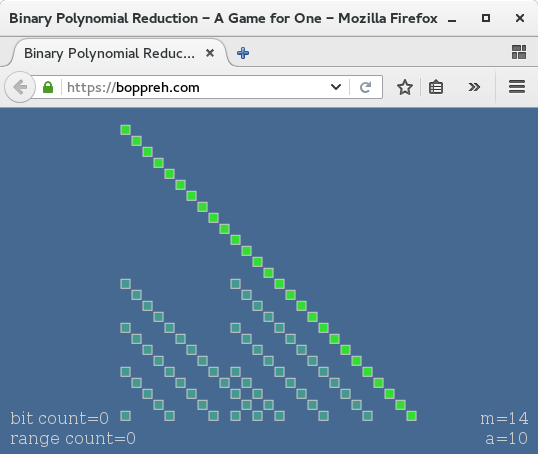
\includegraphics[width = .7\columnwidth]{figures/boppreh.png}
\end{figure}

\begin{figure}
  \caption{Visualization tool with input box for user algorithms.}
  \label{fig:source}
  \centering
  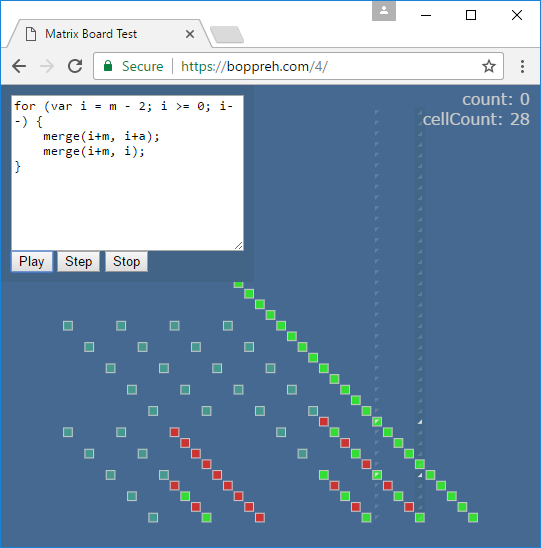
\includegraphics[width = .7\columnwidth]{figures/source.png}
\end{figure}


\section{Algorithm specific visualization}

The previous tools were suited for exploring the behavior of irreducible polynomials when used for reduction. However, we still needed to analyze the specific behavior of our algorithm, such as circuit delay and number of logic gates. \\

To achieve this we created a separate version of the visualizatiom tool where the logic gates connect according to our proposed algorithm. Notice however that the circuit shown is not accurate about the positioning of the logic gates, only their number and connections. \\

Figure~\ref{fig:circuit_reducing_7_3_0} shows the resulting circuit of applying Algorithm~\ref{alg:reduce} to $x^7 + x^3 + 1$. The vertical lines represent the inputs, with the line numbered $i$ representing the coefficient $c_i$ of the polynomial to be reduced. The $\oplus$  connectors perform bit-wise XOR of the upper and left inputs, with the resulting signal on the bottom wire. The numbers at the bottom represent the length of the critical path on that output, a measure proportional do the circuit delay. Note the operations are equivalent to the ones described in Figure~\ref{fig:visual:new}, but with common sub-expression being grouped. \\

\begin{figure}
  \caption{Visualization tool for generated reduction circuits using Algorithm~\ref{alg:reduce}, fixed for the irreducible polynomial $x^7 + x^3 + 1$.}
  \label{fig:circuit_reducing_7_3_0}
  \centering
  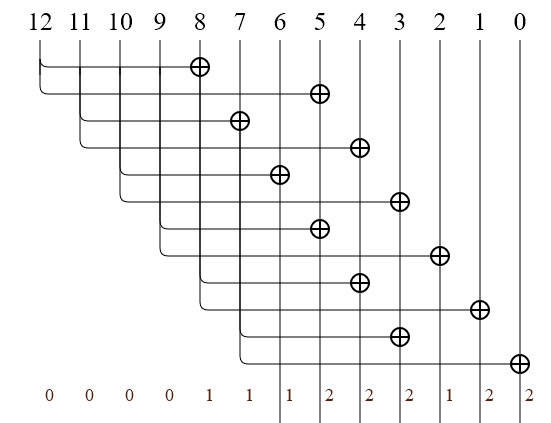
\includegraphics[width = .8\columnwidth]{figures/reducing-7-3-0.png}
\end{figure}

This tool was also adapted for Algorithm~\ref{alg:square}, showing the resulting circuit optimized for squaring in Figure~\ref{fig:circuit_squaring_7_3_0}. Note that the number of operations is much smaller, and that odd-numbered coefficients are skipped. However, in this case the circuit delay remains the same (2 times the delay of a XOR gate). \\

\begin{figure}
  \caption{Visualization tool for generated squaring circuits using Algorithm~\ref{alg:square}, fixed for the irreducible polynomial $x^7 + x^3 + 1$.}
  \label{fig:circuit_squaring_7_3_0}
  \centering
  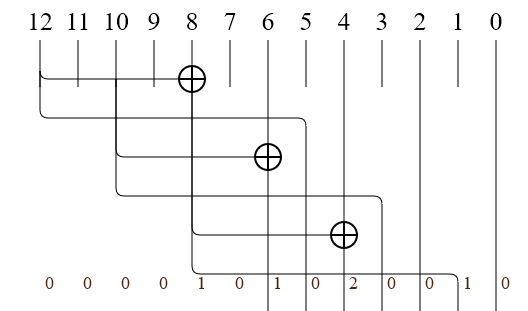
\includegraphics[width = .8\columnwidth]{figures/squaring-7-3-0.png}
\end{figure}

The visualization can be used for any desired polynomial, including pentanomials. In this case the results are naturally more complex, as seen in Figure~\ref{fig:circuit_reducing_7_6_1_0}, which shows a reduction circuit for $x^7 + x^6 + x^2 + x + 1$.

\begin{figure}
  \caption{Visualization tool for generated reduction circuits for the irreducible polynomial $x^7 + x^6 + x^2 + x + 1$.}
  \label{fig:circuit_reducing_7_6_1_0}
  \centering
  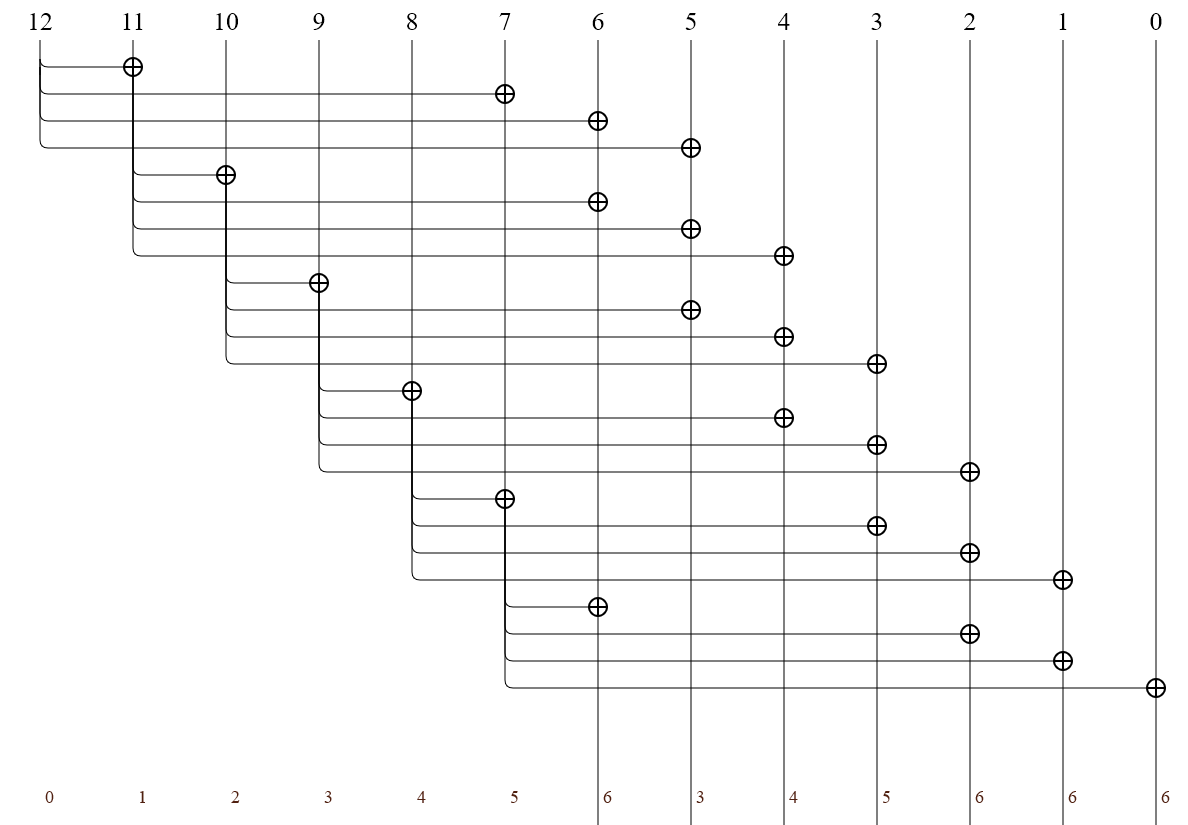
\includegraphics[width = 1\columnwidth]{figures/reducing-7-6-2-1-0.png}
\end{figure}

One of the issues with our proposed algorithm is that the delay is sometimes worse than the state of the art. This can be remediated by moving the connections and inserting extra XOR gates, but doing this analysis by hand is cumbersome. Therefore we added a feature to highlight the gates used on each output, and mark the ones that make up the critical path. This highlighting feature can be seen in Figure~\ref{fig:circuit_reducing_critical_7_6_1_0}, where the 6 XOR gates in the critical path are shown in red. \\

\begin{figure}
  \caption{Visualization tool for generated reduction circuits for the irreducible polynomial $x^7 + x^6 + x^2 + x + 1$. The critical path of output 6 is highlighted.}
  \label{fig:circuit_reducing_critical_7_6_1_0}
  \centering
  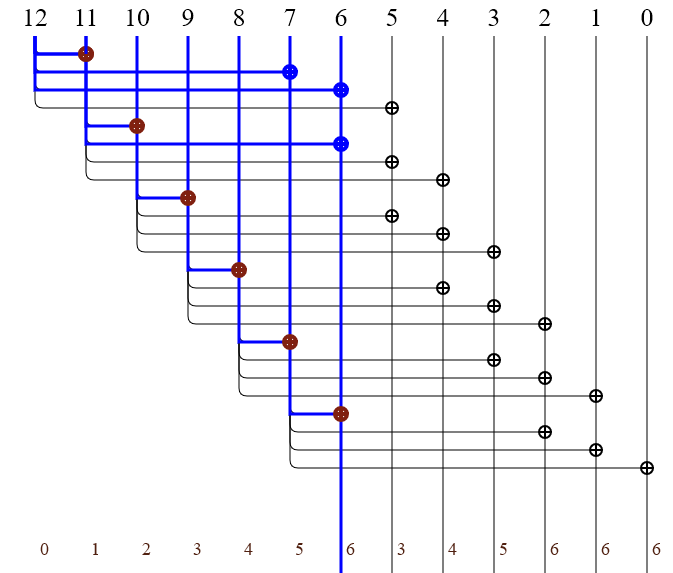
\includegraphics[width = .8\columnwidth]{figures/reducing-critical-7-6-2-1-0.png}
\end{figure}

\section{Conclusion} \label{section:visual:conclusion}

In this chapter we presented the visualization tool used during our research. This tool was invaluable in efficiently exploring and testing new ideas related to reduction of binary polynomials. The intuitive visuals and quick feedback allowed even people unfamiliar with the subjects to help find interesting properties. \\

The development itself of the tool also acted to clarify concepts. For example the fact that each irreducible polynomial has a mathematical "pattern" associated, corresponding to the XORs required for reduction, and that these operations are independent of the algorithm used. The word processing and squaring versions saw less use, but creating them helped guide some of the research. \\

Interestingly, some time after having developed the tool, we found another researcher using the same visualization of patterns, for the same problem~\cite{paper_com_imagens_dos_padroes}. \\

The algorithm-specific version of the visualization tool was also helpful. It lead to deeper insights on the behavior of our proposed algorithm, and to create hand-modified circuits with lower delays.